%set the master document for easy compilation
%!TEX root = ../D3_5_3.tex

\section{DMI}

\subsection{Component Requirements}

\begin{longtable}{p{.25\textwidth}p{.7\textwidth}}
\toprule
Component name			& DMI \\
\midrule
Link to SCADE model		& {\footnotesize \url{https://github.com/openETCS/modeling/tree/master/model/Scade/System/DMI_Control}} \\
\midrule
SCADE designer			& Valerio D'Angelo, DB Netz AG \\
\midrule
Description				& The DMI controller interacts with the DMI display and is responsible for alls procedures between the DMI display and Driver. Furthermore, the DMI controller will interact with the DMI Management to compute the received information (e.g. driver number request, ...) and send, if necessary, data or reports to the DMI Management (acknowledge, text messages...). The DMI Controller is a passive module, this means that all the processing are performed EVC-side, therefore the DMI Controller simply responds to the requests of the EVC or Driver and performs some checks according with the information received from EVC. \\
\midrule
Input documents	& 
ERA\_ERTMS\_015560 \\
\midrule
Safety integrity level	& 4 \\
\midrule
Time constraints		& [If applicable description of time constraints, otherwise n/a] \\
\midrule
API requirements 		& [If applicable description of API requirements, otherwise n/a] \\
\bottomrule
\end{longtable}


\subsection{Interface}

An overview of the interface of component DMI is shown in Figure~\ref{f:DMI_interface}. The inputs and outputs are described in detail in Section~\ref{s:DMI_inputs} respectively \ref{s:DMI_outputs}.

\begin{figure}
\center
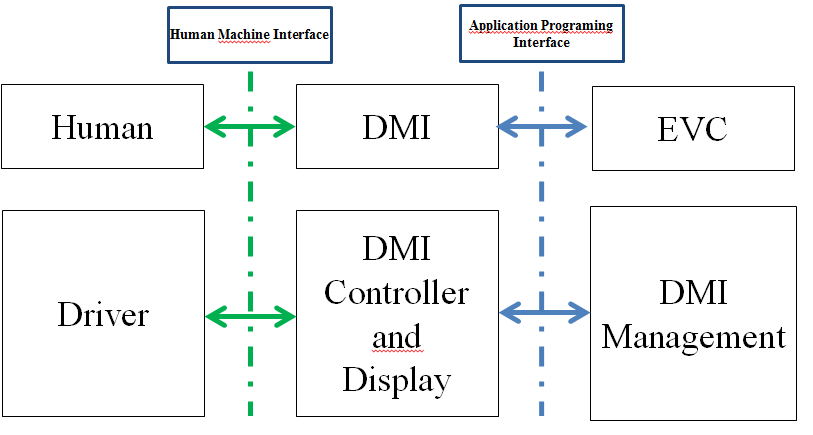
\includegraphics[width=.8\textwidth]{images/DMI_Interfaces}
\caption{DMI component SysML diagram}\label{f:DMI_interface}
\end{figure}


\subsubsection{Inputs}\label{s:DMI_inputs}

\paragraph{DMI\_entry\_request}

\begin{longtable}{p{.25\textwidth}p{.7\textwidth}}
\toprule
Input name				& DMI\_entry\_request \\
\midrule
Description				& Request to input data (e.g. driver id, Train running number etc.) \\
\midrule
Source					& DMI Management \\ 
\midrule
Type					& [Type of the input] \\
\midrule
Valid range of values	& [Complete list of valid values] \\
\midrule
Behaviour when value is at boundary	& [Description of components behaviour when input value is at boundary] \\
\midrule
Behaviour for values out of valid range	& [Description of components behaviour when input value is out of valid range] \\
\midrule
Behaviour when value is erroneous, absent or unwanted (i.e. spurious) & [Description of components behaviour when value is erroneous, absent or unwanted (i.e. spurious)] \\
\bottomrule
\end{longtable}

\paragraph{DMI\_identifier\_request}

\begin{longtable}{p{.25\textwidth}p{.7\textwidth}}
\toprule
Input name				& DMI\_identifier\_request \\
\midrule
Description				& Request of the DMI informations \\
\midrule
Source					& DMI Management \\ 
\midrule
Type					& [Type of the input] \\
\midrule
Valid range of values	& [Complete list of valid values] \\
\midrule
Behaviour when value is at boundary	& [Description of components behaviour when input value is at boundary] \\
\midrule
Behaviour for values out of valid range	& [Description of components behaviour when input value is out of valid range] \\
\midrule
Behaviour when value is erroneous, absent or unwanted (i.e. spurious) & [Description of components behaviour when value is erroneous, absent or unwanted (i.e. spurious)] \\
\bottomrule
\end{longtable}

\paragraph{DMI\_menu\_request}

\begin{longtable}{p{.25\textwidth}p{.7\textwidth}}
\toprule
Input name				& DMI\_menu\_request \\
\midrule
Description				& Request to enable or disable buttons \\
\midrule
Source					& DMI Management \\ 
\midrule
Type					& [Type of the input] \\
\midrule
Valid range of values	& [Complete list of valid values] \\
\midrule
Behaviour when value is at boundary	& [Description of components behaviour when input value is at boundary] \\
\midrule
Behaviour for values out of valid range	& [Description of components behaviour when input value is out of valid range] \\
\midrule
Behaviour when value is erroneous, absent or unwanted (i.e. spurious) & [Description of components behaviour when value is erroneous, absent or unwanted (i.e. spurious)] \\
\bottomrule
\end{longtable}

\paragraph{DMI\_dynamic}

\begin{longtable}{p{.25\textwidth}p{.7\textwidth}}
\toprule
Input name				& DMI\_dynamic \\
\midrule
Description				& Contains informations about current speed, current mode etc. \\
\midrule
Source					& DMI Management \\ 
\midrule
Type					& [Type of the input] \\
\midrule
Valid range of values	& [Complete list of valid values] \\
\midrule
Behaviour when value is at boundary	& [Description of components behaviour when input value is at boundary] \\
\midrule
Behaviour for values out of valid range	& [Description of components behaviour when input value is out of valid range] \\
\midrule
Behaviour when value is erroneous, absent or unwanted (i.e. spurious) & [Description of components behaviour when value is erroneous, absent or unwanted (i.e. spurious)] \\
\bottomrule
\end{longtable}

\paragraph{DMI\_text\_message}

\begin{longtable}{p{.25\textwidth}p{.7\textwidth}}
\toprule
Input name				& DMI\_text\_message \\
\midrule
Description				& Contains predefined or plain text messages \\
\midrule
Source					& DMI Management \\ 
\midrule
Type					& [Type of the input] \\
\midrule
Valid range of values	& [Complete list of valid values] \\
\midrule
Behaviour when value is at boundary	& [Description of components behaviour when input value is at boundary] \\
\midrule
Behaviour for values out of valid range	& [Description of components behaviour when input value is out of valid range] \\
\midrule
Behaviour when value is erroneous, absent or unwanted (i.e. spurious) & [Description of components behaviour when value is erroneous, absent or unwanted (i.e. spurious)] \\
\bottomrule
\end{longtable}

\paragraph{DMI\_icons}

\begin{longtable}{p{.25\textwidth}p{.7\textwidth}}
\toprule
Input name				& DMI\_icons \\
\midrule
Description				& Request to display one or more icons in any area \\
\midrule
Source					& DMI Management \\ 
\midrule
Type					& [Type of the input] \\
\midrule
Valid range of values	& [Complete list of valid values] \\
\midrule
Behaviour when value is at boundary	& [Description of components behaviour when input value is at boundary] \\
\midrule
Behaviour for values out of valid range	& [Description of components behaviour when input value is out of valid range] \\
\midrule
Behaviour when value is erroneous, absent or unwanted (i.e. spurious) & [Description of components behaviour when value is erroneous, absent or unwanted (i.e. spurious)] \\
\bottomrule
\end{longtable}

\paragraph{DMI\_driver\_identifier}

\begin{longtable}{p{.25\textwidth}p{.7\textwidth}}
\toprule
Input name				& DMI\_driver\_identifier \\
\midrule
Description				& Contains the default or entered driver identifier \\
\midrule
Source					& DMI Management \\ 
\midrule
Type					& [Type of the input] \\
\midrule
Valid range of values	& [Complete list of valid values] \\
\midrule
Behaviour when value is at boundary	& [Description of components behaviour when input value is at boundary] \\
\midrule
Behaviour for values out of valid range	& [Description of components behaviour when input value is out of valid range] \\
\midrule
Behaviour when value is erroneous, absent or unwanted (i.e. spurious) & [Description of components behaviour when value is erroneous, absent or unwanted (i.e. spurious)] \\
\bottomrule
\end{longtable}

\paragraph{DMI\_train\_running\_number}

\begin{longtable}{p{.25\textwidth}p{.7\textwidth}}
\toprule
Input name				& DMI\_train\_running\_number \\
\midrule
Description				& Contains the default or entered train running number \\
\midrule
Source					& DMI Management \\ 
\midrule
Type					& [Type of the input] \\
\midrule
Valid range of values	& [Complete list of valid values] \\
\midrule
Behaviour when value is at boundary	& [Description of components behaviour when input value is at boundary] \\
\midrule
Behaviour for values out of valid range	& [Description of components behaviour when input value is out of valid range] \\
\midrule
Behaviour when value is erroneous, absent or unwanted (i.e. spurious) & [Description of components behaviour when value is erroneous, absent or unwanted (i.e. spurious)] \\
\bottomrule
\end{longtable}

\paragraph{DMI\_train\_data}

\begin{longtable}{p{.25\textwidth}p{.7\textwidth}}
\toprule
Input name				& DMI\_train\_data \\
\midrule
Description				& Contains the default or entered train data \\
\midrule
Source					& DMI Management \\ 
\midrule
Type					& [Type of the input] \\
\midrule
Valid range of values	& [Complete list of valid values] \\
\midrule
Behaviour when value is at boundary	& [Description of components behaviour when input value is at boundary] \\
\midrule
Behaviour for values out of valid range	& [Description of components behaviour when input value is out of valid range] \\
\midrule
Behaviour when value is erroneous, absent or unwanted (i.e. spurious) & [Description of components behaviour when value is erroneous, absent or unwanted (i.e. spurious)] \\
\bottomrule
\end{longtable}

\paragraph{TIU\_trainStatus}

\begin{longtable}{p{.25\textwidth}p{.7\textwidth}}
\toprule
Input name				& TIU\_trainStatus \\
\midrule
Description				& Open/close Desk signal \\
\midrule
Source					& TIU \\ 
\midrule
Type					& [Type of the input] \\
\midrule
Valid range of values	& [Complete list of valid values] \\
\midrule
Behaviour when value is at boundary	& [Description of components behaviour when input value is at boundary] \\
\midrule
Behaviour for values out of valid range	& [Description of components behaviour when input value is out of valid range] \\
\midrule
Behaviour when value is erroneous, absent or unwanted (i.e. spurious) & [Description of components behaviour when value is erroneous, absent or unwanted (i.e. spurious)] \\
\bottomrule
\end{longtable}



\subsubsection{Outputs}\label{s:DMI_outputs}

\paragraph{DMI\_identifier}

\begin{longtable}{p{.25\textwidth}p{.7\textwidth}}
\toprule
Output name				& DMI\_identifier \\
\midrule
Description				& Information about DMI (e.g. version, cabin identifier etc.) \\
\midrule
Destination				& DMI Management \\ 
\midrule
Type					& [Type of the output] \\
\midrule
Valid range of values	& [Complete list of valid values] \\
\midrule
Behaviour when value is at boundary	& [Description of components behaviour when output value is at boundary] \\
\midrule
Behaviour for values out of valid range	& [Description of components behaviour when output value is out of valid range] \\
\midrule
Behaviour when value is erroneous, absent or unwanted (i.e. spurious) & [Description of components behaviour when value is erroneous, absent or unwanted (i.e. spurious)] \\
\bottomrule
\end{longtable}

\paragraph{DMI\_driver\_request}

\begin{longtable}{p{.25\textwidth}p{.7\textwidth}}
\toprule
Output name				& DMI\_driver\_request \\
\midrule
Description				& Driver request or acknowledgement \\
\midrule
Destination				& DMI Management \\ 
\midrule
Type					& [Type of the output] \\
\midrule
Valid range of values	& [Complete list of valid values] \\
\midrule
Behaviour when value is at boundary	& [Description of components behaviour when output value is at boundary] \\
\midrule
Behaviour for values out of valid range	& [Description of components behaviour when output value is out of valid range] \\
\midrule
Behaviour when value is erroneous, absent or unwanted (i.e. spurious) & [Description of components behaviour when value is erroneous, absent or unwanted (i.e. spurious)] \\
\bottomrule
\end{longtable}


\paragraph{DMI\_train\_data\_ack}

\begin{longtable}{p{.25\textwidth}p{.7\textwidth}}
\toprule
Output name				& DMI\_train\_data\_ack \\
\midrule
Description				& Train data acknowledgement \\
\midrule
Destination				& DMI Management \\ 
\midrule
Type					& [Type of the output] \\
\midrule
Valid range of values	& [Complete list of valid values] \\
\midrule
Behaviour when value is at boundary	& [Description of components behaviour when output value is at boundary] \\
\midrule
Behaviour for values out of valid range	& [Description of components behaviour when output value is out of valid range] \\
\midrule
Behaviour when value is erroneous, absent or unwanted (i.e. spurious) & [Description of components behaviour when value is erroneous, absent or unwanted (i.e. spurious)] \\
\bottomrule
\end{longtable}


\paragraph{DMI\_status\_report}

\begin{longtable}{p{.25\textwidth}p{.7\textwidth}}
\toprule
Output name				& DMI\_status\_report \\
\midrule
Description				& The actual status of DMI (keep alive) \\
\midrule
Destination				& DMI Management \\ 
\midrule
Type					& [Type of the output] \\
\midrule
Valid range of values	& [Complete list of valid values] \\
\midrule
Behaviour when value is at boundary	& [Description of components behaviour when output value is at boundary] \\
\midrule
Behaviour for values out of valid range	& [Description of components behaviour when output value is out of valid range] \\
\midrule
Behaviour when value is erroneous, absent or unwanted (i.e. spurious) & [Description of components behaviour when value is erroneous, absent or unwanted (i.e. spurious)] \\
\bottomrule
\end{longtable}


\paragraph{DMI\_text\_message\_ack}

\begin{longtable}{p{.25\textwidth}p{.7\textwidth}}
\toprule
Output name				& DMI\_text\_message\_ack \\
\midrule
Description				& Text message acknowledgement \\
\midrule
Destination				& DMI Management \\ 
\midrule
Type					& [Type of the output] \\
\midrule
Valid range of values	& [Complete list of valid values] \\
\midrule
Behaviour when value is at boundary	& [Description of components behaviour when output value is at boundary] \\
\midrule
Behaviour for values out of valid range	& [Description of components behaviour when output value is out of valid range] \\
\midrule
Behaviour when value is erroneous, absent or unwanted (i.e. spurious) & [Description of components behaviour when value is erroneous, absent or unwanted (i.e. spurious)] \\
\bottomrule
\end{longtable}


\paragraph{DMI\_icons\_ack}

\begin{longtable}{p{.25\textwidth}p{.7\textwidth}}
\toprule
Output name				& DMI\_icons\_ack \\
\midrule
Description				& Icon acknowledgement \\
\midrule
Destination				& DMI Management \\ 
\midrule
Type					& [Type of the output] \\
\midrule
Valid range of values	& [Complete list of valid values] \\
\midrule
Behaviour when value is at boundary	& [Description of components behaviour when output value is at boundary] \\
\midrule
Behaviour for values out of valid range	& [Description of components behaviour when output value is out of valid range] \\
\midrule
Behaviour when value is erroneous, absent or unwanted (i.e. spurious) & [Description of components behaviour when value is erroneous, absent or unwanted (i.e. spurious)] \\
\bottomrule
\end{longtable}


\paragraph{DMI\_driver\_identifier}

\begin{longtable}{p{.25\textwidth}p{.7\textwidth}}
\toprule
Output name				& DMI\_driver\_identifier \\
\midrule
Description				&  Contains the default or entered driver identifier \\
\midrule
Destination				& DMI Management \\ 
\midrule
Type					& [Type of the output] \\
\midrule
Valid range of values	& [Complete list of valid values] \\
\midrule
Behaviour when value is at boundary	& [Description of components behaviour when output value is at boundary] \\
\midrule
Behaviour for values out of valid range	& [Description of components behaviour when output value is out of valid range] \\
\midrule
Behaviour when value is erroneous, absent or unwanted (i.e. spurious) & [Description of components behaviour when value is erroneous, absent or unwanted (i.e. spurious)] \\
\bottomrule
\end{longtable}

\paragraph{DMI\_train\_running\_number}

\begin{longtable}{p{.25\textwidth}p{.7\textwidth}}
\toprule
Output name				& DMI\_train\_running\_number \\
\midrule
Description				& Contains the default or entered train running number \\
\midrule
Destination				& DMI Management \\ 
\midrule
Type					& [Type of the output] \\
\midrule
Valid range of values	& [Complete list of valid values] \\
\midrule
Behaviour when value is at boundary	& [Description of components behaviour when output value is at boundary] \\
\midrule
Behaviour for values out of valid range	& [Description of components behaviour when output value is out of valid range] \\
\midrule
Behaviour when value is erroneous, absent or unwanted (i.e. spurious) & [Description of components behaviour when value is erroneous, absent or unwanted (i.e. spurious)] \\
\bottomrule
\end{longtable}

\paragraph{DMI\_train\_data}

\begin{longtable}{p{.25\textwidth}p{.7\textwidth}}
\toprule
Output name				& DMI\_train\_data \\
\midrule
Description				& Contains the default or entered train data \\
\midrule
Destination				& DMI Management \\ 
\midrule
Type					& [Type of the output] \\
\midrule
Valid range of values	& [Complete list of valid values] \\
\midrule
Behaviour when value is at boundary	& [Description of components behaviour when output value is at boundary] \\
\midrule
Behaviour for values out of valid range	& [Description of components behaviour when output value is out of valid range] \\
\midrule
Behaviour when value is erroneous, absent or unwanted (i.e. spurious) & [Description of components behaviour when value is erroneous, absent or unwanted (i.e. spurious)] \\
\bottomrule
\end{longtable}




%\subsection{Sub Components}

%\subsubsection{Management\_of\_Radio\_Communication}
%%set the master document for easy compilation
%!TEX root = ../D3_5_3.tex

\paragraph{Component Requirements}

\begin{longtable}{p{.25\textwidth}p{.7\textwidth}}
\toprule
Component name			& MoRC\_Main\_v2 (Management\_of\_Radio\_Communication) \\
\midrule
Link to SCADE model		& {\footnotesize \url{https://github.com/openETCS/modeling/tree/master/model/Scade/System/ObuFunctions/Radio/MoRC}} \\
\midrule
SCADE designer			& Uwe Steinke, Siemens \\
\midrule
Description				& 
The function \emph{MoRC\_Main\_v2} implements the session states establishing, maintaining and terminating as described in Subset-026, chap. 3.5. A SCADE state machine reflects this state model  accurately. Within each of the states, the activities needed as long as the state is active, are performed. \newline

\emph{MoRC\_Main\_v2} is related to exactly one of the radio mobile modems onboard, monitors its status and controls the processes of registration to the radio network, connecting to one RBC and establishing a radio session with the RBC. \emph{MoRC\_Main\_v2} communicates with its mobile modem directly via the API.  \newline

As the OBU is required to manage up to two RBCs,  two instances of \emph{MoRC\_Main\_v2} are used.  \newline

In addition, \emph{MoRC\_Main\_v2} generates the radio connection indication for the driver.

\\
\midrule
Input documents	& 
Subset-026, Chapter 3.5 \\
\midrule
Safety integrity level		& 4 \\
\midrule
Time constraints		& Implements several time delays, therefore appropriate clocking required \\
\midrule
API requirements 		& Interfaces to the OBUs mobile modem hardware via API \\
\bottomrule
\end{longtable}


\paragraph{Interface}

For an overview of the interface of this internal component we refer to the SCADE model (cf.~link above) respectively the SCADE generated documentation.


